\documentclass[12pt]{report}
\usepackage[pdftex]{graphicx}
\usepackage{url}
\usepackage{amsmath}
\newcommand{\HRule}{\rule{\linewidth}{0.5mm}}
% correct bad hyphenation here
\hyphenation{op-tical net-works semi-conduc-tor auto-nomous}


\begin{document}
%
% paper title
% can use linebreaks \\ within to get better formatting as desired
\title{Design of an Attitude and Heading Reference Sensor}
\author{Patrick Hickey\\pat@moreproductive.org}
\begin{titlepage}
\begin{center}

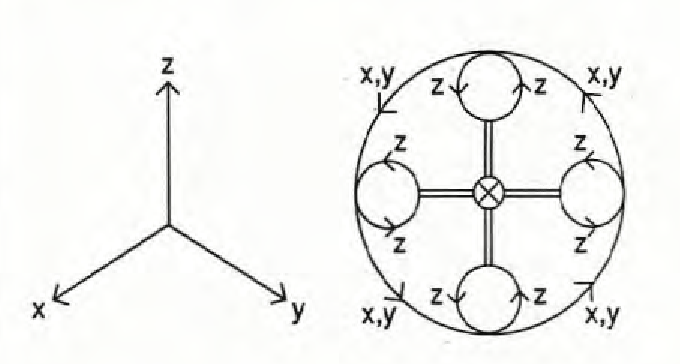
\includegraphics[width=0.3\textwidth]{./cycloid.png}\\[2cm]
\HRule \\[1cm]
{ \huge \bfseries Design of an Attitude and Heading Reference Sensor } \\[1cm]
\HRule \\[0.5cm]
{ \large \bfseries Presented for completion of an Independent Study in Electrical Engineering }
\\[0.5cm]
{ \large \bfseries Rutgers, The State University of New Jersey }
\\[0.5cm]
\HRule \\[1cm]

{\large Pat Hickey}
\\ 
pat@moreproductive.org
\\[0.5cm]
\emph{Advisor}
\\ Dr. Chung-chieh Shan
\\ Department of Computer Science
\vfill
{\large \today}

\end{center}
\end{titlepage}


\begin{abstract}
This paper describes the design of an Attitude and Heading Reference Sensor (AHRS), which measures rootational orientation relative to north and down. 
The design uses 3-axis accellerometer, magnetometer, and rate gyro sensors. 
I will discuss the selection and construction of the sensor hardware, design and implementation of a Kalman filter for sensor fusion, and the test of both the sensor hardware and software.
\end{abstract}


\section{Problem Description}

The goal of this project was to design and build sensor hardware and software that would determine the angular orientation and angular rotation rate of the sensor relative to the earth frame, ie. North, East, and Down. I selected sensor integrated circuits (ICs) which determine, on three axes, body accelleration, body rotation rate, and relative magnetic field. These three sensors (accellerometer, rate gyro, and magnetometer) provide a total of nine measurments. 

An algorithm is required to convert these nine measurments into an expression of angular orientation and angular rate (the derivative, with respect to time, of angular orientation). Angular orientation of a body has three degrees of freedom, as does angular rate. The conversion from measurment space to estimate space (a pair of angular orientation estimate and angular rate estimate) is nonlinear and uses a four-dimensional vector called a quaternion to describe the three-dimensional angular orientation. This is to say, a big part of the problem is ensuring the correctness of this difficult conversion process.   

I selected a well-known algorithm which implements a Quaternion Kalman Filter. This provides an state estimate using the four-dimensional quaternion vector, and an additional three-dimensional rotational rate vector. I needed to implement that software so that I could test it for correctness and use it to determine the orientation of an actual sensor. This software was to be used in an actual model aircraft autopilot system, so it must meet requirments for reliability and soft real-time performance.

\subsection{Application}

As part of my role on the Rutgers Autonomous Aircraft Team, I've been working on a model aircraft autopilot system based on a single board computer which runs Linux \footnote{For more information on this project, see \url{http://moreproductive.org/autopilot/}}. I implemented the control, navigation, and telemetry software in C using standard Linux system calls and threads. I used dedicated hardware for real-time tasks, for example, a microcontroller-based servo controller connected via USB ensures proper servo control despite irregular communication intervals from the computer. 
By using helper threads for input and output, we can be reasonably sure the main control loop will run at close to 60Hz. This is considered ``soft'' real-time.

The sensor software needs to cooperate with the soft real-time main control loop. In order to stabilize an inherently stable fixed-wing aircraft, we need to update the main control loop's orientation estimate at at least 30Hz, preferably at 60Hz. So the sensor hardware must provide new measurments at a rate exceeding 30Hz, a complete measurment every 3.3ms. The sensor filtration software must complete computation in much less than a measurment period as not to dominate the CPU. Lets consider a target time of 500us per computation.

\subsection{Use of Haskell}

The sensor software I describe in this paper is typically implemented in a low level language such as C or C++ in order to give the programmer explicit control over memory allocation and input-output (IO) calls. In fact, open source implementations of very similar software is available. So, in order to make this work in some way novel, I decided to write the filter software using Haskell. Haskell is a purely functional language with a powerful type system, and is not typically used for soft real-time applications.

\section{Theoretical Basis}
\subsection{Measurment Vectors}
\subsubsection{Accellerometer Measurment}

An accellerometer measures force exerted by a small test mass against a beam connected to the sensor body. 

-- Figure here, of a small mass mt on a beam 

The current generation of MEMS accellerometers uses etched silicon to build the test mass and beam structure, and measures the capicatance between the test mass and sensor body to determine the beam deflection.Since an accellerometer can only measure deflection, and therefore accelleration, in one direction, we use three separate sensors oriented to measure accelleration along three orthogonal axes. These three separate measured accellerations ($a_x, a_y, a_z$) can be considered as a three dimensional vector $A = \begin{bmatrix}a_x&a_y&a_z \end{bmatrix}$

According to Newton's second law, $F = m a$ , the force on a body will be directly proportional to the accelleration of the body. When we consider a small test mass $m_t$ on a beam, and the system is at rest, the mass will exert a force $F_g = m_t g_b$, where $g$ is the accelleration due to gravity in the body frame. A body accelleration ab will exert a force $F_a = m_t a_b$. The sensor measures the sum of these two forces, so for any $F = F_g + F_a = m_t ( g_b + a_b )$. Because $m_t$ is constant, we can consider the calibrated measurment 
\begin{equation} 
  A_m = \frac{F}{m_t} = g_b + a_b
\end{equation} 
 
In this application we're interesting in estimating $g_b$ in order to find the vector, in the body frame, which points straight down in the world frame. On a body such as an aircraft, where accellerations may come from any direction at any time, we consider $a_b$ to be a random vector with a covariance matrix 
\begin{equation} Q_a = \begin{pmatrix} \sigma_a^2 & 0 & 0 \\
				                               0 & \sigma_a^2 & 0 \\ 
					                             0 & 0 & \sigma_a^2 \end{pmatrix} 
\end{equation}

We typically estimate a value for $\sigma_a$ to be between 2 and 4$g$ for airborne applications.



\subsubsection{Magnetometer Measurment}

A magnetometer measures 

\subsection{Quaternion Representation}

\subsection{Algorithm Overview}

\section{Hardware}
\subsection{Sensors}
needed 3 axis magnetometer, accellerometer, rate gyro
selected two ics:
invensense itg3200
st micro ...
\subsection{Microcontroller}
uart required to talk to a pc (ttyUSB), i2c required to talk to sensors
arduino pro mini was a simple solution, easy to use programming environment
\subsection{Construction}
provide photographs, schematic


\section{Embedded Software}
\subsection{Requirments}
timing and communication requirments of embedded hardware
st acc self test
\subsection{Communication Protocol}
serial strings etc.
\subsection{Arduino Environment}
describe arduino programming environment
blocking serial calls
-- Provide timing information?

\section{Filtration Software}
The filtration software was implemented in Haskell. The code may be found on Github at \url{http://github.com/pchickey/hs-qkf/}
\subsection{Algorithm Selection}
find an algorithm which assumes my measurment sources
\subsection{Implementation of Filter}
hmatrix-static
quaternions
\subsection{Implementation of Tests}
euler models
rotation-matrix based vector measurment simulation
addition of noise
\subsection{Sensor Interface}
serial.hs
\subsection{Gnuplot Interface}
overview, code snippets
\subsection{OpenGL Demonstration Interface}
cube.hs overview, code snippets 
\subsection{Paparazzi Autopilot Interface}
ffi, linux mq
"ongoing investigation"

\section{Results}
\subsection{Noise-free simulated measurments}
Plots of step test, ramp test
\subsection{Noisy simulated measurments}
step test, ramp test
\subsection{Tests with Sensor}
plots, link to video on youtube

\end{document}


